\documentclass[
11pt,
a4paper,
pdftex,
czech,
titlepage
]{report}

\usepackage[czech]{babel}
\usepackage[utf8]{inputenc}
\usepackage{lmodern}
\usepackage{textcomp}
\usepackage[T1]{fontenc}
\usepackage{amsfonts}
\usepackage{titlesec}
\usepackage{graphicx}
\usepackage[pdftex]{hyperref}
\usepackage[a4paper,left=30mm,right=30mm,top=28mm,bottom=30mm]{geometry}
\usepackage{enumitem}
\usepackage[final]{pdfpages}
\usepackage{listings}
\hypersetup{colorlinks=true,
  unicode=true,
  linkcolor=black,
  citecolor=black,
  urlcolor=black,
  bookmarksopen=true}

\titleformat{\chapter}
  {\normalfont\LARGE\bfseries}{\thechapter}{1em}{}
\titlespacing*{\chapter}{0pt}{0ex plus 1ex minus .2ex}{2.0ex plus .2ex}

\begin{document}

\begin{titlepage}
	%\vspace*{-2cm}
	{\centering
\includegraphics[scale=1.2]{img/logo-FAV.pdf}\par}
	\centering
	\vspace*{2.5cm}
	{\Large Semestrální práce z KIV/DB2\par}
	\vspace{1.5cm}
	{\Huge\bfseries Tradiční piškvorky\par}
	\vspace{2.5cm}

	{\Large Zdeněk Častorál\par}
	{\Large A19N0026P\par}
	{\Large zcastora@students.zcu.cz\par}

	\vfill

	{\Large 12.\,5.\,2020}
\end{titlepage}

\tableofcontents
\thispagestyle{empty}
\clearpage

\newpage
\chapter{Zadání}\label{zadani}
\setcounter{page}{3}
Cílem této práce je navrhnout a vytvořit relační databázi pro hraní známé strategické deskové hry \textit{Piškvorky}. Ze hry bude řešena pouze databázová vrstva aplikace, proto se snažte co nejvíce programových rutin uložit do databáze a také zajistěte jejich automatické spouštění při nastalé události.

Tradiční piškvorky jsou hra pro dva hráče, která se hraje na čtverečkovaném papíře. Ve hře se hráči střídají po jednom tahu, ve kterém každý hráč umístí na volné místo na papíře svoji značku. Obvykle hráči používají symboly kolečko (O) a křížek (X). Vítězí ten hráč, kterému se podaří sestavit nepřerušovanou řadu alespoň pěti svých značek v libovolném směru (vodorovně, svisle, uhlopříčně). Pokud není možné umístit novou značku, hra končí remízou.

Hra probíhá na papíře, který bude mít definovanou velikost. Nejmenší rozměr papíru, na kterém bude možné hrát, může mít rozměry 5x5 čtverečků, největší rozměr papíru nesmí překročit velikost 20x20 čtverečků. Také bude možné definovat, na kolik značek se bude hrát. Velikost vítězné řady by měla být z intervalu 5 až 15. Je třeba si dát pozor na skutečnost, aby se vítězná řada vešla na definovaný papír.

Také se bude měřit herní čas. Hra začíná umístěním první značky začínajícího hráče. V ten samý okamžik se začíná měřit herní čas druhého hráče a to až do doby, kdy umístí svoji značku. Pak se začíná měřit čas začínajícího hráče. Jakmile začínající hráč umístí svoji druhou značku, pozastaví se měření jeho herního času a opětovně se spustí měření času druhého hráče. A tak pořád dokola, až hra skončí výhrou jednoho z hráčů nebo remízou.\\


\begin{figure}[!ht]
	\centering
	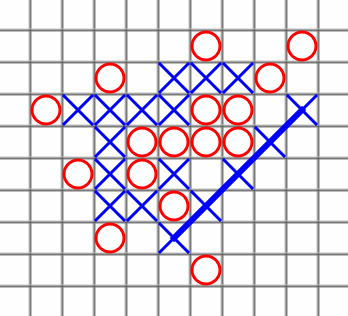
\includegraphics[scale=0.9]{img/tic_tac_toe.png}
	\caption{Piškvorky, Zdroj: \texttt{https://cs.wikipedia.org/wiki/Piškvorky}}
	\label{data_model_obr}
\end{figure}

\subsubsection{V relační databázi budou evidována data v těchto tabulkách:}
\begin{itemize}
    \item \texttt{OMEZENI} -- Tato tabulka slouží jako parametry programu. Obsahuje informace, jak veliký či malý může být čtverečkovaný papír, na kterém se bude hrát a také jak dlouhá či krátká může být minimálně řada symbolů vítězného hráče.
    \item \texttt{STAV} -- Číselník ukazující, v jakém stavu se může nacházet hra. Stavy mohou být tyto: rozehraná, vítězství začínajícího hráče, prohra začínajícího hráče nebo remíza.
    \item \texttt{HRAC} -- Každý hráč, který bude chtít hrát, musí být zaregistrován. Výhodou bude možnost sledovat jeho statistiky hraní, tj. počet vítězství, proher či remíz, a zda začínal nebo hrál jako druhý.
    \item \texttt{HRA} -- Každá hra se hraje na novém čistém papíře o dané velikosti na požadovaný počet vítězných symbolů. Hru hrají dva různí hráči, kde jeden z nich umisťuje kolečka, ten druhý křížky a jeden z nich celou hru začíná. Tabulka bude také obsahovat, v jaké stavu je hra a také herní časy obou hráčů.
    \item \texttt{TAH} -- Umístění své značky hráčem, který je na řadě v rozehrané hře. Ke každému tahu se bude automaticky ukládat časová značka, která dočasně nebo trvale zastavuje měření času právě hrajícímu hráči.
\end{itemize}

\subsubsection{Z uložených dat v databázi vytvořte databázové pohledy, které nabídnou tato data:}
\begin{itemize}
    \item \begin{sloppypar}\texttt{PAPIR} -- Zobrazení čtverečkovaného papíru obsahující všechny dosud provedené tahy právě probíhající hry. Každý řádek papíru bude zobrazen voláním funkce \texttt{RADEK\_PAPIRU}.
    \end{sloppypar}
    \item \texttt{VYHRY\_ZACINAJICI} -- Hry, ve kterých zvítězil začínající hráč. Obsahuje parametry hry (rozměry papíru, požadovaná velikost vítězné řady), jména hráčů, kdo začínal (a zvítězil), kdo používal jaké značky, jak dlouho celá hra trvala v sekundách, kolik bylo zahráno tahů.
    \item \texttt{PROHRY\_ZACINAJICI} -- Hry, ve kterých prohrál začínající hráč. Obsahuje parametry hry (rozměry papíru, požadovaná velikost vítězné řady), jména hráčů, kdo začínal (a prohrál), kdo používal jaké značky, jak dlouho celá hra trvala v sekundách, kolik bylo zahráno tahů.
    \item \texttt{REMIZY} -- Hry, které dospěly do remízy. Obsahuje parametry hry (rozměry papíru, požadovaná velikost vítězné řady), jména hráčů, kdo začínal, kdo používal jaké značky, jak dlouho celá hra trvala v sekundách.
\end{itemize}

V databázových pohledech \texttt{VYHRY\_ZACINAJICI}, \texttt{PROHRY\_ZACINAJICI} a \texttt{REMIZY} získejte dobu hraní hry jako součet herních dob obou hráčů.


\subsubsection{V databázi budou uloženy a používány tyto funkce (s parametry):}
\begin{itemize}
    \item \texttt{SPATNY\_PARAMETR} -- Podle návratové hodnoty funkce poznáme, že je:
    \begin{itemize}
        \item 0 - vše v pořádku.
        \item 1 - příliš malý počet řádků na papíru (menší než 5).
        \item 2 - příliš velký počet řádků na papíru (větší než 20).
        \item 3 - příliš malý počet sloupců na papíru (menší než 5).
        \item 4 - příliš velký počet sloupců na papíru (větší než 20).
        \item 5 - příliš malý počet znaků ve vítězné řadě (menší než 5).
        \item 6 - příliš velký počet znaků ve vítězné řadě (větší než 15).
        \item 7 - vítězná řada delší, než šířka papíru.
        \item 8 - vítězná řada delší, než výška papíru.
    \end{itemize}

    \item \texttt{RADEK\_PAPIRU} -- Vrátí řetězec, který odpovídá konkrétnímu řádku papíru dané hry. Pro výpis zvolte v řetězci tyto symboly:
    \begin{itemize}
        \item \texttt{X} - značka křížek jednoho hráče dané hry.
        \item \texttt{O} - značka kolečko druhého hráče hry.
        \item \texttt{mezera} - symbol označující volné políčko na papíře.
    \end{itemize}
    \item \texttt{HERNI\_CAS} -- Vrátí číslo určující, kolik sekund hrál daný hráč danou hru, tj. sečte rozdíly časových značek, kdy hrál daný hráč a kdy hrál před ním druhý hráč.
    \item \texttt{REMIZA} -- Vrátí hodnotu \texttt{TRUE}, pokud daná hra dospěla do remízového stavu, tj. není možné udělat další tah. Jinak vrací hodnotu \texttt{FALSE}.
    \item \texttt{VYHRA} -- Vrátí hodnotu \texttt{TRUE}, pokud právě hrající hráč v dané hře vyhrál, tj. svým posledním tahem docílil požadované minimální délky vítězné řady svých značek. Jinak vrací hodnotu \texttt{FALSE}.
\end{itemize}

\subsubsection{V databázi budou uloženy a jako těla triggerů používány tyto procedury (s parametry):}
\begin{itemize}
    \item \texttt{ZABRAN\_HRE} -- Zabrání vytvoření nové hry, pokud je nastaven špatně libovolný parametr hry.
    \item \texttt{ZABRAN\_TAHU} -- Zabrání tahu, který není možno udělat.
    \item \texttt{KONEC\_HRY} -- Spočítání herních časů hráčů právě dokončené hry.
    \item \texttt{STATISTIKY} -- Aktualizace statistických údajů hráčů, kteří dohráli danou hru.
\end{itemize}

\subsubsection{O automatické činnosti v databázi se postarají triggery o:}
\begin{itemize}
    \item hlídání parametrů nové hry (volání funkce \texttt{SPATNY\_PARAMETR}),
    \item hlídání hráčů, aby se ve hře pravidelně střídali po jednom tahu,
    \item hlídání hráče, aby nepokládal svoji značku na již obsazené místo,
    \item hlídání hráče, aby nemohl realizovat tah ve hře, ve které nehraje,
    \item hlídání hráče, aby nemohl realizovat tah ve hře, která již skončila,
    \item hlídání a aktualizace stavu hry, tj. zda nedospěla do remízy nebo vítězství jednoho z hráčů (volání funkcí \texttt{REMIZA} a \texttt{VYHRA}),
    \item spočítání herní doby hráčů, kteří dohráli aktuální hru (volání funkce \texttt{HERNI\_CAS}),
    \item aktualizace statistických údajů hráčů, kteří dohráli aktuální hru.
\end{itemize}

\subsubsection{Konfigurace, spuštění a průběh hry}
\begin{enumerate}
    \item Jednorázová konfigurace databáze:
    \begin{enumerate}
        \item Naplnění tabulky \texttt{OMEZENI} hraničními hodnotami parametrů nové hry.
        \item Naplnění tabulky \texttt{STAV} daty odpovídající různým stavům hry.
    \end{enumerate}
    \item Registrace hráčů je provedena vkládáním nových záznamů do tabulky \texttt{HRAC}.
    \item Hra je zahájena úspěšným vložením nového záznamu do tabulky \texttt{HRA}. Neúspěšné vložení znamená, že některé parametry hry jsou mimo hraniční hodnoty definované v tabulce \texttt{OMEZENI}.
    \item Že hra běží, ověříme zobrazením papíru, tj. vypsáním řádků prostřednictvím databázového pohledu \texttt{PAPIR} pro aktuálně rozehranou hru.
    \item Každý tah ve hře je proveden vložením nového záznamu do tabulky \texttt{TAH}. Pokud ke vložení nedošlo, byla aktivována některá z výše uvedených kontrol.
    \item Po úspěšném tahu je vhodné si vždy zobrazit aktuální situaci na papíře prostřednictvím databázového pohledu \texttt{PAPIR}.
    \item Pokud hra neskončila, pokračuj bodem 5, jinak bodem 8 (výhra) nebo bodem 9 (remíza).
    \item Hra skončila vítězstvím jednoho z hráčů. To je vhodné ověřit voláním pohledu \texttt{VYHRY\_ZACINAJICI} nebo \texttt{PROHRY\_ZACINAJICI} a také se podívat na aktualizované statistiky hrajících hráčů v tabulce \texttt{HRAC}. Jdi na bod 10.
    \item Hra skončila remízou. To je vhodné ověřit voláním pohledu \texttt{REMIZY} a také se podívat na aktualizované statistiky hrajících hráčů v tabulce \texttt{HRAC}.
    \item Novou hru zahájíme bodem 3, s případnou registrací nového hráče bodem 2.
\end{enumerate}

\chapter{Datový model}\label{data_model}
Datový model obsahuje pět tabulek. Jedná se o tabulky:
\begin{itemize}
    \item OMEZENI -- tato tabulka slouží jako parametry programu,
    \item STAV -- číselník, který ukazuje, v jakém stavu se může hra nacházet,
    \item HRAC -- tato tabulka obsahuje registrované hráče a jejich statistiky,
    \item HRA -- tato tabulka obsahuje jednotlivé hry (včetně aktuálního stavu hry a herních časů obou hráčů),
    \item TAH -- tabulka, která obsahuje jednotlivé tahy umístěné hráčem, který je na řadě v rozehrané hře.
\end{itemize}

Detailní specifikace tabulek je uvedena v kapitole \ref{zadani}. Datový model včetně atributů je uveden na obrázku \ref{data_model_obr}.

\begin{figure}[!ht]
	\centering
	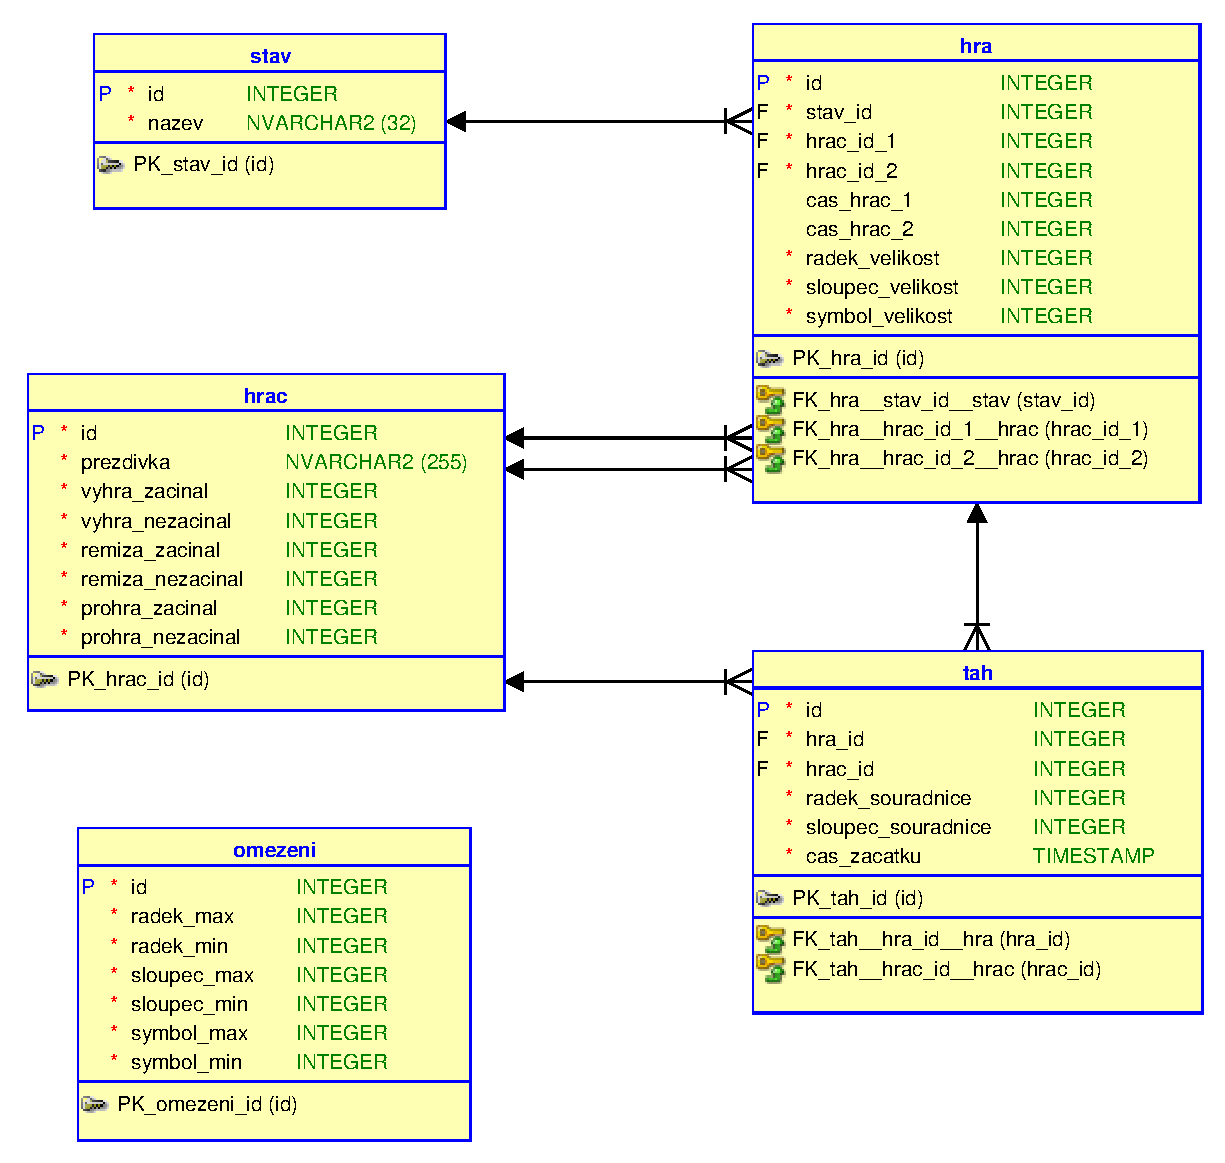
\includegraphics[width=1\textwidth]{img/data_model.pdf}
	\caption{Datový model}
	\label{data_model_obr}
\end{figure}

\chapter{Implementace}\label{implementace}
Implementace byla provedena prostřednictvím jazyka \texttt{PL/SQL} v prostředí databáze \texttt{Oracle} verze \texttt{19c}.

V této kapitole je popsána implementace jednotlivých databázových objektů, jejichž detailní specifikace a analýza je uvedena v kapitole \ref{zadani}.

\section{Tabulky}
Tabulky byly implementovány v souladu s datovým modelem popsaným v kapitole \ref{data_model}. V~kapitole \ref{tab_tah} je podrobněji popsána implementace tabulky \texttt{TAH}.\\

\noindent Skript pro vytvoření všech tabulek je uložen v souboru:
\begin{center}
\noindent \framebox{\texttt{src\textbackslash01\_create\_scripts\textbackslash01\_create\_tables.sql}}\\[0.5\baselineskip]
\end{center}

\subsection{\texttt{TAH}}\label{tab_tah}
Tabulka \texttt{TAH} obsahuje jednotlivé tahy umístěné hráčem, který je na řadě v rozehrané hře. Atribut \texttt{hrac\_id} specifikuje hráče, který umístil daný tah ve hře, která je specifikovaná atributem \texttt{hra\_id}. Atribut \texttt{cas\_zacatku} ukládá časovou značku, která reprezentuje začátek měření herního času oponenta. V~definici tabulky je časová značka generována automaticky při vložení nového záznamu prostřednictvím klíčových slov \texttt{DEFAULT CURRENT\_TIMESTAMP}. 

Implementace tabulky \texttt{TAH} včetně přidání primárních a cizích klíčů zobrazuje ukázka kódu \ref{tah_kod}.



\lstset{language=SQL, numbers=left, frame=single, caption=Vytvoření tabulky \texttt{TAH},  breaklines=true, basicstyle=\small\ttfamily, commentstyle=\itshape, keywordstyle=\bfseries, tab=~, tabsize=2, xleftmargin=5mm, xrightmargin=5mm, label=tah_kod}
\renewcommand{\lstlistingname}{Ukázka kódu}
\begin{lstlisting}
CREATE TABLE tah (
    id                   INTEGER NOT NULL,
    hra_id               INTEGER NOT NULL,
    hrac_id              INTEGER NOT NULL,
    radek_souradnice     INTEGER NOT NULL,
    sloupec_souradnice   INTEGER NOT NULL,
    cas_zacatku          TIMESTAMP DEFAULT CURRENT_TIMESTAMP NOT NULL
);

ALTER TABLE tah ADD CONSTRAINT pk_tah_id PRIMARY KEY ( id );

ALTER TABLE tah
    ADD CONSTRAINT fk_tah__hra_id__hra FOREIGN KEY ( hra_id )
        REFERENCES hra ( id );

ALTER TABLE tah
    ADD CONSTRAINT fk_tah__hrac_id__hrac FOREIGN KEY ( hrac_id )
        REFERENCES hrac ( id );
\end{lstlisting}


\section{Funkce}
V~databázi byly implementovány všechny požadované funkce uvedené v kapitole \ref{zadani}. Dále byla implementována pomocná funkce \texttt{VYKRESLI\_PAPIR}, která slouží k vykreslení všech řádků papíru dané hry a je nutná k implementaci pohledu \texttt{PAPIR} (podrobněji viz kapitola \ref{pohled_papir_kap}). Pro shrnutí, databáze obsahuje funkce:
\begin{itemize}
    \item \texttt{RADEK\_PAPIRU} -- vrací řetězec, který odpovídá konkrétnímu řádku papíru dané hry,
    \item \texttt{VYKRESLI\_PAPIR} -- vrací řetězec, který odpovídá všem řádkům papíru dané hry (podrobněji v kapitole \ref{vykresli_papir_kap}),
    \item \texttt{VYHRA} -- vrací hodnotu \texttt{TRUE}, pokud právě hrající hráč v dané hře vyhrál, jinak vrací \texttt{FALSE},
    \item \texttt{REMIZA} -- vrací hodnotu \texttt{TRUE}, pokud daná hra dospěla do remízového stavu, jinak vrací \texttt{FALSE},
    \item \texttt{HERNI\_CAS} -- vrací číslo, které určuje, kolik sekund hrál daný hráč danou hru,
    \item \texttt{SPATNY\_PARAMETR} -- vrací číslo podle konkrétní chyby v nastavení hry.
\end{itemize}

\noindent Skript pro vytvoření všech funkcí je uložen v souboru:
\begin{center}
\noindent \framebox{\texttt{src\textbackslash01\_create\_scripts\textbackslash02\_create\_functions.sql}}\\[1\baselineskip]
\end{center}

\subsection{\texttt{VYKRESLI\_PAPIR}}\label{vykresli_papir_kap}
Jak již bylo zmíněno výše, funkce \texttt{VYKRESLI\_PAPIR} vrací řetězec, který odpovídá všem řádkům papíru dané hry. Tato funkce je volána v pohledu \texttt{PAPIR} (viz kapitola \ref{pohled_papir_kap}). 

Tato funkce pro zadané \texttt{id} hry volá ve smyčce funkci \texttt{RADEK\_PAPIRU} pro každý řádek dané hry. Zřetězení všech výstupních řetězců funkce \texttt{RADEK\_PAPIRU} je vráceno jako výsledný řetězec funkce \texttt{VYKRESLI\_PAPIR}. Implementace této funkce je zobrazena v ukázce kódu \ref{vykresli_papir_kod}.

\lstset{language=SQL, numbers=left, frame=single, caption=Implementace funkce \texttt{VYKRESLI\_PAPIR},  breaklines=true, basicstyle=\small\ttfamily, commentstyle=\itshape, keywordstyle=\bfseries, tab=~, tabsize=2, xleftmargin=5mm, xrightmargin=5mm, label=vykresli_papir_kod}
\renewcommand{\lstlistingname}{Ukázka kódu}
\begin{lstlisting}
CREATE OR REPLACE FUNCTION vykresli_papir ( hra_id IN INTEGER ) RETURN NVARCHAR2 AS
hra_radek hra%ROWTYPE;
papir_vypis NVARCHAR2(2100) := '';   

BEGIN
    SELECT * INTO hra_radek 
    FROM hra 
    WHERE hra.id = hra_id
        AND rownum = 1;

    FOR aktualni_radek IN 1..hra_radek.radek_velikost LOOP
        papir_vypis := papir_vypis|| radek_papiru ( hra_radek.id, aktualni_radek )|| chr(10);
    END LOOP;
    
    RETURN papir_vypis;
END;
/
\end{lstlisting}

\section{Procedury}
V~databázi byly implementovány všechny požadované procedury uvedené v kapitole \ref{zadani}. Navíc byla implementována procedura \texttt{AKTUALIZUJ\_STAV\_HRY}, která aktualizuje stav dokončené hry, a pomocné procedury \texttt{REGISTRUJ\_HRACE}, \texttt{ZAHAJ\_HRU}, \texttt{PROVED\_TAH}. Databáze tedy obsahuje procedury:

\begin{itemize}
    \item \texttt{KONEC\_HRY} -- procedura spočítá herní časy hráčů právě dokončené hry (podrobněji v kapitole \ref{konec_hry_kap}),
    \item \texttt{AKTUALIZUJ\_STAV\_HRY} -- tato procedura aktualizuje stav dokončené hry (podrobněji v kapitole \ref{aktual_stav_kap}),
    \item \texttt{STATISTIKY} -- aktualizuje statistické údaje hráčů, kteří dohráli danou hru,
    \item \texttt{ZABRAN\_HRE} -- zabrání vytvoření nové hry, pokud je nastaven špatně některý z parametrů hry,
    \item \texttt{ZABRAN\_TAHU} -- zabrání tahu, který není možné udělat,
    \item \texttt{REGISTRUJ\_HRACE} -- pomocná procedura pro registraci hráče (podrobněji v kapitole \ref{reg_hrace_kap}),
    \item \texttt{ZAHAJ\_HRU} -- pomocná procedura pro zahájení nové hry,
    \item \texttt{PROVED\_TAH} -- pomocná procedura pro realizaci tahu.
\end{itemize}

\noindent Skript pro vytvoření všech procedur je uložen v souboru:
\begin{center}
\noindent \framebox{\texttt{src\textbackslash01\_create\_scripts\textbackslash03\_create\_procedures.sql}}\\[1\baselineskip]
\end{center}

\subsection{\texttt{KONEC\_HRY}}\label{konec_hry_kap}
Procedura \texttt{KONEC\_HRY} je volána při ukončení hry (tzn. výhře jednoho z hráčů, či remíze) z triggeru \texttt{VYHODNOT\_STAV\_HRY} (viz kapitola \ref{vyhodnot_stav_kap}). Tato procedura spočítá herní časy zúčastněných hráčů prostřednictvím funkce \texttt{HERNI\_CAS} a tyto časy uloží do odpovídajících atributů \texttt{cas\_hrac\_1} a \texttt{cas\_hrac\_2} tabulky \texttt{HRA}. Implementace této procedury je zobrazena v ukázce kódu \ref{konec_hry_kod}.

\lstset{language=SQL, numbers=left, frame=single, caption=Implementace procedury \texttt{KONEC\_HRY},  breaklines=true, basicstyle=\small\ttfamily, commentstyle=\itshape, keywordstyle=\bfseries, tab=~, tabsize=2, xleftmargin=5mm, xrightmargin=5mm, label=konec_hry_kod}
\renewcommand{\lstlistingname}{Ukázka kódu}
\begin{lstlisting}
CREATE OR REPLACE PROCEDURE konec_hry ( hra_id IN INTEGER, hrac_id IN INTEGER ) AS

hra_radek hra%ROWTYPE;
    
BEGIN

    SELECT * INTO hra_radek 
    FROM hra 
    WHERE hra.id = hra_id
        AND rownum = 1;
        
    UPDATE hra
    SET 
        cas_hrac_1 = herni_cas ( hra_radek.id, hra_radek.hrac_id_1 ),
        cas_hrac_2 = herni_cas ( hra_radek.id, hra_radek.hrac_id_2 )
    WHERE id = hra_radek.id;

END;
/
\end{lstlisting}

\subsection{\texttt{AKTUALIZUJ\_STAV\_HRY}}\label{aktual_stav_kap}
\begin{sloppypar}
Procedura \texttt{AKTUALIZUJ\_STAV\_HRY} je také volána při ukončení hry z triggeru \texttt{VYHODNOT\_STAV\_HRY} (viz kapitola \ref{vyhodnot_stav_kap}). Tato procedura aktualizuje stav dokončené hry (tj. zda hra skončila vítězstvím začínajícího hráče, prohrou začínajícího hráče, či remízou) a uloží jej do atributu \texttt{stav\_id} tabulky \texttt{HRA}. Implementace této procedury je zobrazena v ukázce kódu \ref{aktual_stav_kod}.
\end{sloppypar}

\lstset{language=SQL, numbers=left, frame=single, caption=Implementace procedury \texttt{AKTUALIZUJ\_STAV\_HRY},  breaklines=true, basicstyle=\small\ttfamily, commentstyle=\itshape, keywordstyle=\bfseries, tab=~, tabsize=2, xleftmargin=5mm, xrightmargin=5mm, label=aktual_stav_kod}
\renewcommand{\lstlistingname}{Ukázka kódu}
\begin{lstlisting}
CREATE OR REPLACE PROCEDURE aktualizuj_stav_hry ( hra_id IN INTEGER, hrac_id IN INTEGER DEFAULT NULL ) AS

hrac_id_prvni_tah INTEGER;
hra_id_prom INTEGER := hra_id;
    
BEGIN
    IF hrac_id IS NULL THEN
    
        UPDATE hra
        SET stav_id = 4
        WHERE id = hra_id_prom;
        
    ELSE
    
        SELECT t1.hrac_id INTO hrac_id_prvni_tah
        FROM tah t1
		WHERE t1.id = 
			( SELECT MIN(t2.id) FROM tah t2 WHERE t2.hra_id = hra_id_prom );
        
        IF hrac_id_prvni_tah = hrac_id THEN
            
            UPDATE hra
            SET stav_id = 2
            WHERE id = hra_id_prom;
                
        ELSE
        
            UPDATE hra
            SET stav_id = 3
            WHERE id = hra_id_prom;
        
        END IF;
        
    END IF;
END;
/
\end{lstlisting}

\subsection{\texttt{REGISTRUJ\_HRACE}}\label{reg_hrace_kap}
Tato procedura byla vytvořena k usnadnění registrace hráče. Po jejím zavolání s příslušnými parametry dojde vložení nového záznamu do tabulky \texttt{HRAC}. Její implementace je zobrazena v ukázce kódu \ref{reg_hrace_kod}.

\lstset{language=SQL, numbers=left, frame=single, caption=Implementace procedury \texttt{REGISTRUJ\_HRACE},  breaklines=true, basicstyle=\small\ttfamily, commentstyle=\itshape, keywordstyle=\bfseries, tab=~, tabsize=2, xleftmargin=5mm, xrightmargin=5mm, label=reg_hrace_kod}
\renewcommand{\lstlistingname}{Ukázka kódu}
\begin{lstlisting}
CREATE OR REPLACE PROCEDURE registruj_hrace ( prezdivka IN NVARCHAR2, id IN INTEGER DEFAULT NULL ) AS

BEGIN

    IF id IS NULL THEN
        INSERT INTO hrac 
            ( prezdivka, vyhra_zacinal, vyhra_nezacinal, remiza_zacinal, remiza_nezacinal, prohra_zacinal, prohra_nezacinal ) 
        VALUES 
            ( prezdivka, 0, 0, 0, 0, 0, 0 );
    ELSE
        INSERT INTO hrac 
            ( id, prezdivka, vyhra_zacinal, vyhra_nezacinal, remiza_zacinal, remiza_nezacinal, prohra_zacinal, prohra_nezacinal ) 
        VALUES 
            ( id, prezdivka, 0, 0, 0, 0, 0, 0 );
    END IF;
    
    COMMIT;

END;
/
\end{lstlisting}


\section{Pohledy}
Implementované pohledy odpovídají zadání (viz kapitola \ref{zadani}). V~kapitole \ref{pohled_papir_kap} je podrobněji popsána implementace pohledu \texttt{PAPIR}, v kapitole \ref{vyhry_zac_kap} je popsána implementace pohledu \texttt{VYHRY\_ZACINAJICI}.\\

\noindent Skript pro vytvoření všech pohledů je uložen v souboru:
\begin{center}
\noindent \framebox{\texttt{src\textbackslash01\_create\_scripts\textbackslash04\_create\_views.sql}}\\[0.5\baselineskip]
\end{center}

\subsection{\texttt{PAPIR}}\label{pohled_papir_kap}
Pohled \texttt{PAPIR} reprezentuje čtverečkovaný papír obsahující všechny dosud provedené tahy právě probíhající hry. Pohled nebylo možné realizovat pouze s využitím klauzule \texttt{SELECT}, jeho obsah je proto získáván voláním funkce \texttt{VYKRESLI\_PAPIR} (viz kapitola \ref{vykresli_papir_kap}). Tato funkce vyžaduje jako vstupní parametr \texttt{id} hry, pro kterou chceme zobrazit čtverečkovaný papír. Tento parametr je nutné přímo zadat do pohledu \texttt{PAPIR}, jelikož v databázovém systému \texttt{Oracle} nelze vytvořit pohledy s parametry. Implementace tohoto pohledu je zobrazena v ukázce kódu \ref{papir_kod}.

\lstset{language=SQL, numbers=left, frame=single, caption=Implementace pohledu \texttt{PAPIR},  breaklines=true, basicstyle=\small\ttfamily, commentstyle=\itshape, keywordstyle=\bfseries, tab=~, tabsize=2, xleftmargin=5mm, xrightmargin=5mm, label=papir_kod}
\renewcommand{\lstlistingname}{Ukázka kódu}
\begin{lstlisting}
CREATE OR REPLACE VIEW papir AS
    SELECT vykresli_papir(101) AS "Papir"
    FROM dual;
\end{lstlisting}

\subsection{\texttt{VYHRY\_ZACINAJICI}}\label{vyhry_zac_kap}
Tento pohled zobrazí všechny hry, ve kterých zvítězil začínající hráč. Obsahuje parametry hry (rozměry papíru, požadovaná velikost vítězné řady), jména hráčů, kdo začínal (a zvítězil), kdo používal jaké značky, jak dlouho celá hra trvala v sekundách, kolik bylo zahráno tahů. Implementace pohledu \texttt{VYHRY\_ZACINAJICI} je zobrazena v ukázce kódu \ref{vyhry_zac_kod}.

\lstset{language=SQL, numbers=left, frame=single, caption=Implementace pohledu \texttt{VYHRY\_ZACINAJICI},  breaklines=true, basicstyle=\small\ttfamily, commentstyle=\itshape, keywordstyle=\bfseries, tab=~, tabsize=2, xleftmargin=5mm, xrightmargin=5mm, label=vyhry_zac_kod}
\renewcommand{\lstlistingname}{Ukázka kódu}
\begin{lstlisting}
CREATE OR REPLACE VIEW vyhry_zacinajici AS
    SELECT
        h.radek_velikost AS "Pocet radku",
        h.sloupec_velikost AS "Pocet sloupcu",
        h.symbol_velikost AS "Pocet vyhernich symbolu",
        hrac1.prezdivka AS "Hrac 1",
        hrac2.prezdivka AS "Hrac 2",
        
        CASE
            WHEN
                (   (   
                        SELECT t1.hrac_id
                        FROM tah t1
                        WHERE t1.id = 
                            ( SELECT MIN(t2.id) FROM tah t2 WHERE t2.hra_id = h.id )
                    ) = hrac1.id
                 )
            THEN
                hrac1.prezdivka
            ELSE
                hrac2.prezdivka
        END AS "Zacinal (zvitezil)",
        
        'O' AS "Hrac 1 - symbol",
        'X' AS "Hrac 2 - symbol",
        h.cas_hrac_1 + h.cas_hrac_2 AS "Trvani hry",
        
        (   
            SELECT COUNT(t.id)
            FROM tah t
            WHERE t.hra_id = h.id
        ) AS "Pocet tahu"
        
    FROM hra h
        INNER JOIN hrac hrac1 ON hrac1.id = h.hrac_id_1
        INNER JOIN hrac hrac2 ON hrac2.id = h.hrac_id_2
    WHERE h.stav_id = 2;
\end{lstlisting}

\section{Triggery}
V aplikaci byly implementovány tři triggery, které splňují požadovanou funkcionalitu a automatizaci činností v databázi (viz kapitola \ref{zadani}). Těmito triggery jsou:
\begin{itemize}
    \item \texttt{VYHODNOT\_STAV\_HRY} -- trigger, který hlídá a vyhodnotí stav hry, tj. zda nedospěla do remízy, nebo vítězného stavu jednoho z hráčů (podrobněji v kapitole \ref{vyhodnot_stav_kap}),
    \item \texttt{ZKONTROLUJ\_PARAMETRY\_HRY} -- hlídá parametry nové hry při vytvoření, jestli splňují daná omezení,
    \item \texttt{ZKONTROLUJ\_TAH\_HRACE} -- hlídá platnost tahu hráče.
\end{itemize}

\noindent Skript pro vytvoření všech triggerů je uložen v souboru:
\begin{center}
\noindent \framebox{\texttt{src\textbackslash01\_create\_scripts\textbackslash05\_create\_triggers.sql}}\\[1\baselineskip]
\end{center}

\subsection{\texttt{VYHODNOT\_STAV\_HRY}}\label{vyhodnot_stav_kap}
Trigger \texttt{VYHODNOT\_STAV\_HRY} hlídá a vyhodnocuje stav hry, zda nedospěla do konečného stavu. 

Tento trigger vyhodnocuje stav hry po každém novém tahu, tj. vložení nového záznamu do tabulky \texttt{TAH}. Z nového záznamu je nutné získat souřadnice nového symbolu a vyhodnotit, zda hra nedospěla do vítězství jednoho z hráčů, či remízy. Nicméně, použití \textit{řádkového triggeru} \texttt{AFTER INSERT} na tabulku \texttt{TAH} není v tomto případě možné. Funkce \texttt{VYHRA}, která stav hry vyhodnocuje, kontroluje záznamy v tabulce \texttt{TAH}, ale nový záznam ještě není ve chvíli spuštění triggeru v této tabulce obsažen (příkaz \texttt{COMMIT} po vložení nového záznamu do tabulky tah je vykonán až po vykonání triggeru). Samotné použití \textit{příkazového triggeru} \texttt{AFTER INSERT} na tabulku \texttt{TAH} také není možné. Příkazový trigger je sice vykonán až po klauzuli \texttt{COMMIT}, nicméně už z jeho podstaty není možné přímo přistupvat k novému záznamu prostřednictvím pseudozáznamu \texttt{:new}.

Řešením je použít tzv. \texttt{COMPOUND TRIGGER}, v jehož těle lze definovat všechny čtyři typy triggerů (příkazový \texttt{BEFORE}, řádkový \texttt{BEFORE}, řádkový \texttt{AFTER}, příkazový \texttt{AFTER}). Trigger \texttt{VYHODNOT\_STAV\_HRY} je právě \texttt{COMPOUND TRIGGER} nad tabulkou \texttt{TAH} pro operaci \texttt{INSERT}. 
\begin{sloppypar}
V tomto triggeru jsou definovány globální proměnné \texttt{hra\_id\_prom} (\texttt{id} hry, ve které je nový tah realizován) a \texttt{hrac\_id\_prom} (\texttt{id} hráče, který nový tah realizoval). V sekci \texttt{AFTER\_EACH\_ROW} (řádkový trigger) je umožněn přístup k pseudozáznamu \texttt{:new} a hodnoty nového řádku jsou v této sekci přiřazeny do definovaných globálních proměnných. V sekci \texttt{AFTER STATEMENT} (příkazový trigger) jsou vykonány kontroly stavu hry, kde díky globálním proměnným jsou hodnoty nového záznamu známé. Implementace tohoto triggeru je zobrazena v ukázce kódu \ref{vyhodnot_stav_kod}.\end{sloppypar}

\lstset{language=SQL, numbers=left, frame=single, caption=Implementace triggeru \texttt{VYHODNOT\_STAV\_HRY},  breaklines=true, basicstyle=\small\ttfamily, commentstyle=\itshape, keywordstyle=\bfseries, tab=~, tabsize=2, xleftmargin=5mm, xrightmargin=5mm, label=vyhodnot_stav_kod}
\renewcommand{\lstlistingname}{Ukázka kódu}
\begin{lstlisting}
CREATE OR REPLACE TRIGGER vyhodnot_stav_hry
    FOR INSERT ON tah
    COMPOUND TRIGGER
    
    hra_id_prom INTEGER;
    hrac_id_prom INTEGER;
    
    AFTER EACH ROW IS
    BEGIN
    
        hra_id_prom := :new.hra_id;
        hrac_id_prom := :new.hrac_id;
        
    END AFTER EACH ROW;
    
    AFTER STATEMENT IS
    BEGIN
    
        IF vyhra ( hra_id_prom, hrac_id_prom ) THEN
            konec_hry ( hra_id_prom, hrac_id_prom );
            aktualizuj_stav_hry ( hra_id_prom, hrac_id_prom );
            statistiky ( hra_id_prom );
        END IF;
    
        IF remiza ( hra_id_prom ) THEN
            konec_hry ( hra_id_prom, hrac_id_prom );
            aktualizuj_stav_hry ( hra_id_prom );
            statistiky ( hra_id_prom );
        END IF;
    
    END AFTER STATEMENT;

    
END vyhodnot_stav_hry;
/
\end{lstlisting}

\chapter{Nasazení aplikace}\label{nasazeni}
Databázová aplikace byla realizována a testována pro prostředí databáze \texttt{Oracle} verze \texttt{19c} a vyšší.

\section{Struktura souborů aplikace}
Kořenový adresář aplikace obsahuje:
\begin{itemize}
    \item adresář \texttt{doc} -- dokumentace aplikace (vč. jejích zdrojových souborů),
    \item adresář \texttt{model} -- datový model databáze (vč. souborů k editaci),
    \item adresář \texttt{src} -- zdrojové soubory aplikace v jazyce \texttt{PL/SQL},
    \item soubor \texttt{README.md} -- obsahuje základní informace o aplikaci (např. jak oskriptovat databázi).
\end{itemize}

\subsection{Adresář \texttt{src}}
Zdrojové soubory aplikace jsou v adresáři \texttt{src} rozděleny do podadresářů:
\begin{itemize}
    \item \texttt{01\_create\_scripts} -- skripty k založení všech potřebných databázových objektů (tabulky, funkce, procedury, pohledy, triggery),
    \item \texttt{02\_init\_data\_scripts} -- konfigurační data (naplnění tabulek \texttt{OMEZENI} a \texttt{STAV}),
    \item \texttt{03\_scenario\_scripts} -- testovací scénáře.
\end{itemize}

\section{Skriptování databáze}
Při skriptování databáze je nutné spouštět skripty v následujícím pořadí:
\begin{enumerate}
    \item adresář \texttt{src\textbackslash01\_create\_scripts\textbackslash}:
    \begin{enumerate}
        \item \texttt{01\_create\_tables.sql} -- vytvoří tabulky a sekvence,
        \item \texttt{02\_create\_functions.sql} -- vytvoří databázové funkce,
        \item \texttt{03\_create\_procedures.sql} -- vytvoří databázové procedury,
        \item \texttt{04\_create\_views.sql} -- vytvoří databázové pohledy,
        \item \texttt{05\_create\_triggers.sql} -- vytvoří triggery v databázi,
    \end{enumerate}
    \item adresář \texttt{src\textbackslash02\_init\_data\_scripts\textbackslash}:
        \begin{enumerate}
        \item \texttt{01\_insert\_init\_data} -- naplní databázi konfiguračními daty (tabulky \texttt{OMEZENI} a \texttt{STAV}).
    \end{enumerate}
\end{enumerate}

Po dokončení běhu všech výše uvedených skriptů jsou v databázi založeny všechny potřebné objekty a konfigurační data, v~tuto chvíli je možné databázovou aplikaci používat.


\chapter{Testovací scénáře}\label{test_scenare}
Testovací scénáře jsou uloženy v adresáři \texttt{src\textbackslash03\_scenario\_scripts\textbackslash} v~podadresářích:
\begin{itemize}
    \item \texttt{01\_wrong\_parameters} -- obsahuje testovací scénáře pro zadání špatných parametrů hry a tahu,
    \item \texttt{02\_win\_first} -- obsahuje testovací scénáře pro výhru začínajícího hráče,
    \item \texttt{03\_lose\_first} -- obsahuje testovací scénáře pro prohru začínajícího hráce,
    \item \texttt{04\_tie} -- obsahuje testovací scénáře pro remízu,
    \item \texttt{05\_win\_directions} -- obsahuje testovací scénáře, zda hra dospěla do vítězného stavu v~jednotlivých směrech.
\end{itemize}


\chapter{Závěr}\label{zaver}
Cílem této práce bylo navrhnout a vytvořit relační databázovou aplikaci pro hraní známé strategické deskové hry Piškvorky. V databázové aplikaci jsem implementoval všechny databázové objekty popsané v zadání (kapitola \ref{zadani}). Také jsem vytvořil testovací scénáře (viz kapitola \ref{test_scenare}), které automaticky otestují funkčnost aplikace, včetně chybových stavů. 

Při implementaci jsem se setkal se dvěma výraznějšími problémy. Prvním problémem byla implementace pohledu \texttt{PAPIR}, který nebylo možné realizovat pouze s využitím klauzule \texttt{SELECT}, a proto jsem musel pro vykreslení papíru vytvořit pomocnou funkci. Druhým problémem bylo chování řádkového \texttt{AFTER INSERT} triggeru, místo něhož jsem nakonec použil \texttt{COMPOUND TRIGGER}.\\

\noindent Semestrální práce z mého pohledu splňuje požadavky zadání.

\end{document}